\documentclass[american,a4paper,12pt]{article}
\usepackage[T1]{fontenc} %for å bruke æøå
\usepackage[utf8]{inputenc}
\usepackage{minted}
\usepackage{graphicx} %for å inkludere grafikk
\usepackage{verbatim} %for å inkludere filer med tegn LaTeX ikke liker
\usepackage{algorithm} % for algoritmene e.g paragraf 2.2 Gauss
\usepackage{algpseudocode} % lager pseudokode til algoritmene
\usepackage{caption}
\usepackage{physics}
\usepackage{multicol}
\usepackage{siunitx}
\usepackage{float}
\usepackage{subcaption}
\usepackage{hyperref}
%\usepackage{biblatex}

\hypersetup{
    colorlinks=true,
    linkcolor=black,
    filecolor=magenta,
    urlcolor=blue,
    citecolor=blue
    %pdftitle={Project 1: Computational Physics - FYS3150},
    %pdfpagemode=FullScreen
}

\renewcommand{\vec}[1]{\mathbf{#1}} %ny definisjon av \vec så det blir bold face i stedet for vector-pil.


\captionsetup[table]{skip=10pt}
%\bibliographystyle{plain}

%\bibliographystyle{plain}


%\title{Exploring the buckling beam problem and quantum harmonic potentials with one or two electrons using the Jacobi method }
\title{Using the Jacobi Method to solve eigenvalue problems of the buckling beam and quantum dots}
\author{Fredrik Hoftun \& Mikkel Metzsch Jensen}
\date{\today}
\begin{document}
\maketitle

\begin{abstract}
    In this project we used the Jacobi method to solve eigenvalue problems. We initially looked at the classical problem of the buckling beam, with analytical eigenpairs, which served as a test for the implementation in c++ and use of the Jacobi method. Later on we scaled the equations of the buckling beam problem in order to extend the problem to one or two electrons moving in a three-dimensional harmonic oscillator potential (quantum dots). We saw that the Jacobi algorithm were able to calculate the eigenvalues and eigenvectors successfully for both the buckling beam and quantum dots problem. The Jacobi method turned out to be quite ineffective though considering both run time and precision. It was precise and fast enough for our needs in this project, but compared to the more advanced eigenvalue solver from armadillo (eig\_sym) it lacked behind:
    \begin{align*}
        &E_{\text{Jacobi}}(N) \approx \mathcal{O}(N^{3.2})&  &T_{\text{Jacobi}}(N) \approx \mathcal{O}(N^{3.7})& \\
        &E_{\text{armadilo}} \approx \mathcal{O}(N^{2})& &T_{\text{armadillo}}(N) \approx \mathcal{O}(N^{1.8})&
    \end{align*}


\end{abstract}
\vfill
\footnotesize{{Link to our GitHub repository: \url{https://github.com/mikkelme/project2_FYS3150}}} 
\newpage


\section{Introduction}
In this project we present a numerical approach for solving eigenvalue problems based on Jacobi's method. The eigenvalue problem occurs and play an important role in a wide range of scientific fields, 
and can be very demanding and even impossible to solve analytical for many cases. As we shall see in this project, we will find use of the eigenvalue solver for both classical and quantum mechanics respectively with and without analytical solutions. We are going to take the two-point boundary value problem of a buckling beam (or a spring fastened at both ends) as a starting point of our investigation. This can be rewritten as a eigenvalue problem on the form $\vec{A}u = \lambda u$, where $\vec{A}$ is symmetrical and tridiagonal. Although the Jacobi method can be used on any strictly diagonally dominant system of linear equations, we will limit ourselves to the eigenvalue problem for at symmetrical tridiagonal matrix. We will use the available analytical solutions (eigenvalues and eigenvectors) in order to test and verify the Jacobi method. In addition we are going to implement unit-testing along the way, which shall ensure that the algorithm passes certain mathematical criteria. Once this is done, we will scale the equations from the buckling beam problem such that we can describe the quantum mechanical problem of electrons moving in a three-dimensional harmonic oscillator potential. With the use of the Jacobi method and an implement eigenvalue solver from Armadillo (eig\_sym)\cite{arma}. We are then able to study the role of the repulsive Coulomb interaction which provides interesting physics results. For selected frequencies, this interacting two-electron problem exhibits analytical solutions, which we can use for reference.
\section{Method}
\subsection{The buckling beam problem, a classical wave function problem in one dimension}
The initial problem of this paper is the so-called "buckling beam problem" which deals with the the "bending" of a beam under load. The problem is stated mathematically as the following differential equation:
\begin{equation}
    \gamma \frac{d^2u}{dx^2} = -Fu(x)
    \label{eq:diff_beam}
\end{equation}
The beam has length $L$, $x \in [0,L]$, and the force is applied at the end of the beam $(L,0)$ in the direction towards the origin (squeezing it). $u(x)$ is then the displacement of the beam in the y direction (see figure \ref{fig:buckling_beam}). The parameter $\gamma$ is defined by the properties of the beam (like rigidity). We apply Dirichlet boundary conditions as $u(0) = u(L) = 0$, since we assume that the end points of the beam are fixed.
\begin{figure}[H]
    \centering
    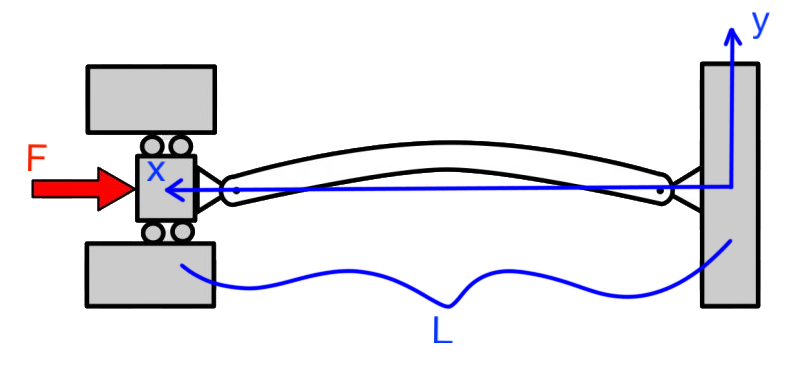
\includegraphics[width = 0.9\textwidth]{figures/buckling_beam.png}
    \caption{Figure for visualizing the buckling beam problem. This is an edited version on a original figure from Wikipedia \footnote{\url{https://en.wikipedia.org/wiki/Buckling#/media/File:Buckled_column.svg}}}
    \label{fig:buckling_beam}
\end{figure}
 We assume that we know $L$ and $F$, and that the eigenvalue problem we set up will allow us to find $\gamma$. We define the dimensional variable:
\begin{align*}
     \rho = \frac{x}{L}
\end{align*}
such that we now have $\rho \in [0,1]$. We then reorder equation \ref{eq:diff_beam} in terms of $\rho$:
\begin{align*}
     \frac{d^2u(\rho)}{d\rho^2} &= - \frac{FL^2}{\gamma}u(\rho) \\
     &= \ \ \ -\lambda \ \ \ u(\rho)
\end{align*}
with $\lambda = FL^2/\gamma$ as our eigenvalue. We discretize $\rho$ in N points as:
\begin{align*}
    \rho_i = \rho_0 + ih \quad \quad i = 1, 2, \hdots, N 
\end{align*}
where
\begin{align*}
    \rho_0 = 0, \quad \rho_N = 1, \quad h = \frac{\rho_N - \rho_0}{N}
\end{align*}
By using the same second derivative approximation as used in project 1 \cite{project1} we get the following equation:
\begin{align*}
    u''(\rho_i) \approx \frac{u(\rho_i + h) - 2u(\rho_i) + u(\rho_i - h)}{h^2} =- \lambda u(\rho_i)
\end{align*}
$\Longleftrightarrow$
\begin{align*}
    -\frac{u_{u+1} - 2u_i + u_{i-1}{h^2}}{h^2} =   \lambda u_i
\end{align*}
By following the same approach as in project 1 \cite{project1} we can express this as a set of linear equations, but this time as a eigenvalue problem:
\begin{equation}
     \begin{bmatrix}
        d & a & 0 & 0 & \cdots & 0 & 0 \\
        a & d & a & 0 & \cdots & 0 & 0 \\
        0 & a & d & a & 0 & \cdots & 0 \\
        \cdots & \cdots & \cdots & \cdots & \cdots & \cdots & \cdots \\
        0 & \cdots & \cdots & \cdots & a & d & a \\
        0 & \cdots & \cdots & \cdots & \cdots & a & d \\
    \end{bmatrix}
    \begin{bmatrix}
    u_1 \\
    u_2 \\
    u_3 \\
    \vdots \\
    u_{N-2} \\
    u_{N-1}
    \end{bmatrix}
    = \lambda
    \begin{bmatrix}
    u_1 \\
    u_2 \\
    u_3 \\
    \vdots \\
    u_{N-2} \\
    u_{N-1}
    \end{bmatrix}
    \label{eq:buckling_beam}
\end{equation}
with definitions:
\begin{align*}
    a = -\frac{1}{h^2}, \quad d = \frac{2}{h^2}
\end{align*}
Note that we do not include the endpoints $u_0$ and $u_N$ here as they are known. This eigenvalue problem have analytical eigenpairs, with eigenvalues: 
\begin{equation}
    \lambda_j = d + 2a \cos{(\frac{j\pi}{N})}, \quad j = 1,2,\hdots, N-1
    \label{eq:analytical_eigvals}
\end{equation}
and eigenvectors:
\begin{equation}
    \vec{u}_j = [\sin{(\frac{j\pi}{N})}, sin(\frac{2j\pi}{N}), \hdots, \sin{\frac{(N-1)j\pi}{N}}]^T, \quad j = 1,2, \hdots N-1
    \label{eq:analytical_eigvecs}
\end{equation}
\cite{project_description}

\subsection{Jacobi method for solving eigenvalue problems}
The Jacobi method is an iterative algorithm for solving strictly diagonally dominant systems of linear equations \cite{wiki:jacobi}. This means that we must demand that the diagonal element is larger than the off-diagonal elements on each row. This is the case given by equation \ref{eq:buckling_beam}, and we can in addition simplify the algorithm by using that the matrix $\vec{A}$ are real and symmetric. For a real symmetric matrix there exists a real orthogonal matrix $\vec{S}$ such that:
\begin{align*}
    \vec{S^T}\vec{A}\vec{S} = \text{diag}(\lambda_1, \lambda_2, \hdots, \lambda_n)
\end{align*}
where $\lambda_1, \lambda_2, \hdots, \lambda_n$ are the eigenvalues (not necessary distinct). In order to obtain these eigenvalues we will use a series of similarity transformations on $\vec{A}$, in order to reduce it into a diagonal form as above. The reason for this lies in the fact that similarity transformations of a matrix does not change the eigenvalues, only the eigenvectors. We say that $\vec{B}$ is a similarity transform of $\vec{A}$ when:
\begin{align*}
    \vec{B} = \vec{S^T}\vec{A}\vec{S}, \qquad \vec{S^T}\vec{S} = \vec{S}^{-1}\vec{S} = \vec{I}
\end{align*}
\\
For the Jacobi rotation we will use a $(n \times n)$ orthogonal transformation matrix:
\begin{align*}
    S = 
    \begin{pmatrix}
        1 & 0 & \cdots & 0 & 0 & \cdots & 0 & 0 \\
        0 & 1 & \cdots & 0 & 0 & \cdots & 0 & 0 \\
        \cdots & \cdots & \cdots & \cdots & \cdots & \cdots & 0 & \cdots \\
        0 & 0 & \cdots & \cos{\theta} & 0 & \cdots & 0 & \sin{\theta} \\
        0 & 0 & \cdots & 0 & 1 & \cdots & 0 & 0 \\
        \cdots & \cdots & \cdots & \cdots & \cdots & \cdots & 1 & \cdots \\
         0 & 0 & \cdots & -\sin{\theta} & 0 & \cdots & 0 & \cos{\theta} \\
    \end{pmatrix}
\end{align*}
where $\vec{S^T} = \vec{S^-1}$. This performs a plane rotation around an angle $\theta$ in the Euclidean n-space. For a given index $l$ and $k$ ($1 \le k < l \le n$) we have the following non zero elements in $\vec{S}$:
\begin{align*}
    s_{ii} = 1, \quad s_{kk} = s_{ll} = \cos{\theta}, \quad s_{kl} = -\sin{\theta}, \quad s_{lk} = \sin{\theta}, \quad i \ne k \  i \ne l
\end{align*}
In order to get the best convergence of the algorithm we will aim to choose $k$ and $l$ such that $a_{kl} = a_{lk}$ is the largest off-diagonal elements. Note that it is beyond the scope of this paper to prove this.  Performing a similarity transformation $\vec{B} = \vec{S^T}\vec{A}\vec{S}$ will then results in the following elements:
\begin{align*}
    b_{ii} &= a_{ii},  \quad i \ne k, i \ \ne l\\
    b_{ik} &= a_{ik}\cos{\theta} - a_{il}\sin{\theta}, \quad i \ne k, i \ \ne l\\
    b_{il} &= a_{il}\cos{\theta} + a_{ik}\sin{\theta}, \quad i \ne k, i \ \ne l\\
    b_{kk} &= a_{kk}\cos^2{\theta} - 2a_{kl}\cos{\theta}\sin{\theta} + a_{ll}\sin^2{\theta} \\
    b_{ll} &= a_{ll}\cos^2{\theta} + 2a_{kl}\cos{\theta}\sin{\theta} + a_{kk}\sin^2{\theta} \\
    b_{kl} &= b{lk} = (a_{kk} - a_{ll})\cos{\theta}\sin{\theta} + a_{kl}(\cos^2{\theta} - \sin^2{\theta})
\end{align*}
Note that we still maintain symmetry such that $b_{ij} = b_{ji}$ for any given $i, j \in [1,N-1]$. The angle $\theta$ is arbitrary and should be chosen so that the off-diagonal matrix elements $b_{kl} = b_{lk}$ becomes zero. We continue this process by choosing new values for $l$ and $k$ (biggest off-diagonal elements) and performing a new similarity transformation $\vec{C} = \vec{S^T}\vec{B}\vec{S}$ to put $c_{kl} = c_{lk} = 0$. Therefore the main idea is to systematically reduce the norm of the off-diagonal elements of the matrix $\vec{A}$:
\begin{align*}
    \text{off}(\vec{A}) = \sqrt{\sum_{i=1}^n\sum_{j=1,j\ne i}^n a^2_{ij}}
\end{align*}
Ideally this should become zero, but because some of the matrix elements which were previously set to zero, may change to non-zero values in the next rotation, it is better to define a tolerance $\epsilon$ which we want $\text{off}(\vec{A})$ to converge to. Since calculating $\text{off}(\vec{A})$ is rather time consuming we can replace it with the simpler criteria for stopping the algorithm: 
\begin{align*}
    \text{max}_{i \ne j}(a_{ij})^2 \le \epsilon
\end{align*}
In order to reach this criteria we have to solve the equation:
\begin{align*}
    b_{kl} = (a_{kk} - a_{ll})\cos{\theta}\sin{\theta} + a_{kl}(\cos^2{\theta} - \sin^2{\theta})= 0
\end{align*}
for $\cos{\theta}$ and $\sin{\theta}$ for each rotation. By using the abbreviations:
\begin{align*}
    c = \cos{\theta}, \quad s = \sin{\theta}, \quad t = \tan{\theta}
\end{align*}
we can simplify this to:
\begin{align*}
    b_{kl} = (a_{kk} - a_{ll})cs + a_{kl}(c^2 - s^2)= 0
\end{align*}
$\Longleftrightarrow$
\begin{align*}
    \frac{a_{kk} - a_{ll}}{a_{kl}}t + 1 - t^2 = 0
\end{align*}
We then define $\tau = (a_{kk} - a_{ll})/2a_{kl}$ which lead to the quadratic form:
\begin{align*}
    -2\tau t + 1 - t^2 = 0 \quad \Longleftrightarrow \quad t^2 + 2\tau t - 1 = 0
\end{align*}
This gives us the solution:
\begin{align*}
    t = -\tau \pm \sqrt{\tau^2 + 1}
\end{align*}
In order to get the fastest convergence we should choose the smallest t. It is beyond the scope of this article to derive this, but i can easily been seen by writing out the calculations for a  2 x 2 matrix (see \cite{lecnotes7}). This means that we choose the plus-sign for $\tau \ge 0$ and minus-sign for $\tau < 0$. When then largest off-diagonal $a_{kl}$ eventually gets smaller and smaller, due to the effect of multiple rotations, we will see that $\tau$ becomes larger. Because of the limitations of numerical precision for large $\tau$ this yields:
\begin{align*}
    t &= -\tau + \sqrt{\tau^2 + 1} = 0, \quad \text{for} \ \tau \rightarrow \infty \\ 
    t &= -\tau - \sqrt{\tau^2 + 1} = 0, \quad \text{for} \ \tau \rightarrow -\infty
\end{align*}
Note that by infinity we mean a large number like $10^{15}$ or higher. In order avoid this computational error we will simply
rewrite the expression. \\ \\
For $\tau \ge 0$ we get: 
\begin{align*}
    t &= \frac{-\tau + \sqrt{\tau^2 + 1}(\tau + \sqrt{\tau^2 + 1})}{\tau + \sqrt{\tau^2 + 1}} \\
     &= \frac{1}{\tau + \sqrt{\tau^2 + 1}}
\end{align*}
and for $\tau < 0$:
\begin{align*}
    t &= \frac{-1}{-\tau + \sqrt{\tau^2 + 1}}
\end{align*}
Here a large $\pm \tau$ will yield $t \ne 0$ in computational practice also. By using common relations between the trigonometric functions we can obtain c and s as:
\begin{align*}
    c = \frac{1}{\sqrt{1+ t^2}}, \qquad s = ct
\end{align*}
The flow of the Jacobi algorithm on our matrix $\vec{A}$ will look something like this:
\begin{itemize}
    \item Choose tolerance $\epsilon$
    \item while $\text{max}(a_{ij})^2 > \epsilon$:
        \begin{itemize}
            \item Choose largest off-diagonal matrix element $a_{kl}$ such that $|a_{kl}| = \text{max}_{i \ne j}|a_{ij}|$
            \item Compute:
                \begin{align*}
                    & \qquad \qquad \tau = \frac{a_{ll} - a_{kk}}{2a_{kl}}&  &\tan{\theta}= \frac{1}{\tau + \sqrt{\tau^2 + 1}}& \\ 
                    & \qquad \qquad \cos{\theta} = \frac{1}{\sqrt{1+ t^2}}&  &\sin{\theta} = ct&
                \end{align*}
            \item Compute similarity transformation using this set of values including $k$ and $l$ such that the new matrix $\vec{A_{new}} = \vec{S^T}\vec{A}\vec{S}$ is obtained. We let the new matrix override the old one immediately since we do not need to save the other.
            \end{itemize}
    \item This continues until $\text{max}(a_{ij})^2 > \epsilon$ is achieved. 
\end{itemize}
In order to obtain the eigenvectors alongside we have to mind the transformations done to the matrix during the rotations. The spectral theorem for symmetric matrices states that a symmetrical matrix $\vec{A}$, is orthogonally diagonalizable such that:
\begin{align*}
    A = \vec{P}\vec{D}\vec{P^T}
\end{align*}
with \vec{P} consisting of normalized eigenvectors of \vec{A} as columns. This means that after performing enough rotations such that the \vec{A} is diagonalized we get
\begin{align*}
    \vec{D} = (\vec{S_1}\vec{S_2}\hdots\vec{S_N})^T\vec{A}(\vec{S_1}\vec{S_2}\hdots\vec{S_N})
\end{align*}
where
\begin{align*}
    P \approx \vec{S_1}\vec{S_2}\hdots\vec{S_N}
\end{align*}
If we keep track of all the rotations we can then essentially read off the eigenvectors of A as the columns of our approximate matrix $\vec{P}$. We do this by initializing a identity matrix and then updating it for every rotation as $\vec{P_new} = \vec{S^T}\vec{A}\vec{S}$. This means essentially  that we have to implement the following operations:
\begin{align*}
    P(i,k) = P(i,k)\cos{\theta} - P(i,l)\sin{\theta};
    P(i,l) = P(i,k)\sin{\theta} + P(i,l)\cos{\theta};
\end{align*}
\\
As a quick test of this method, we chose a tolerance $\epsilon = 10^{-10}$, and implement the explained workflow into c++. we get the following eigenvalues as showed in table \ref{tab:5x5_testing}:
\begin{table}[H]
  \begin{center}
  \caption{Eigenvalue problem of the buckling beam with dimensions $N = 5$ solved with the Jacobi Method and compared to analytical solution \ref{eq:analytical_eigvals}.}
  \begin{tabular}{|c|c|c|c|} \hline
  \textbf{Eigenvalue number} & \textbf{Jacobi Method} & \textbf{Analytical} & \textbf{Absolute Error} \\ \hline     
    1 &            6.69873 &             6.69873 &         8.88178e-15 \\ \hline
    2 &                 25 &                  25 &         1.77636e-14 \\ \hline
    3 &                 50 &                  50 &         3.55271e-14 \\ \hline
    4 &                 75 &                  75 &         5.68434e-14 \\ \hline
    5 &            93.3013 &             93.3013 &         7.10543e-14 \\ \hline
  \end{tabular}
  \label{tab:5x5_testing}
  \end{center}
\end{table}
In addition we get the following numerical eigenvectors
\begin{align*}
    &\vec{v_1} = \begin{bmatrix} 0.29 \\ 0.5 \\ 0.58 \\ 0.5 \\ 0.29                             \end{bmatrix}&
    &\vec{v_2} = \begin{bmatrix} 0.5 \\ 0.5 \\ \num{-1.1e-13} \\ -0.5 \\ -0.5                         \end{bmatrix}&
    &\vec{v_3} = \begin{bmatrix} 0.58 \\ \num{-5.0e-16} \\ -0.58 \\ \num{6.19e-16} \\ 0.58      \end{bmatrix}&
    &\vec{v_4} = \begin{bmatrix} 0.5 \\ -0.5 \\ \num{1.3e-16} \\ 0.5 \\ -0.5                    \end{bmatrix}&
    &\vec{v_5} = \begin{bmatrix} 0.29 \\ -0.5 \\ 0.58 \\ -0.5 \\ 0.8                            \end{bmatrix}& \\
\end{align*} 
Where the analytical eigenvalues (from equation \ref{eq:analytical_eigvecs}) are:
\begin{align*}
     &\vec{v_1} = \begin{bmatrix} 0.5 \\ 0.87 \\ 1 \\ 0.87 \\ 0.5                                \end{bmatrix}&
    &\vec{v_2} = \begin{bmatrix} 0.87 \\ 0.87 \\ \num{1.2e-16} \\ -0.87 \\ -0.87                \end{bmatrix}&
    &\vec{v_3} = \begin{bmatrix} 1 \\ \num{1.2e-16} \\ -1 \\ \num{-2.4e-16} \\ 1                \end{bmatrix}&
    &\vec{v_4} = \begin{bmatrix} 0.87 \\ -0.87 \\ \num{-2.4e-16} \\ 0.87 \\ -0.87               \end{bmatrix}&
    &\vec{v_5} = \begin{bmatrix} 0.5 \\ -0.87 \\ 1 \\ -0.87 \\ 0.5                              \end{bmatrix}&
\end{align*}
By scaling these a bit and realizing that small numbers $< \num{1e-13}$ basically can be seen as zero, these match quite well. By multiplying original matrix $\vec{A}$ with the eigenvectors found by the by the Jacobi method, we can verify that the eigenvectors and eigenvalues are indeed true. This is therefore implemented as a unit-test after a an ended run with the Jacobi method.\\
Other unit-tests we have chosen are one that checks that the algorithm preserves the orthogonality and one that checks that it finds the larges off-diagonal element.

\subsection{Expanding the eigenvalue problem for Quantum dots in three dimensions}
For systems affected by a spherically symmetric potential we can separate the 3D Schröedinger equation (in spherical coordinates) into two equations, the radial- and angular equation. The radial equation in only dependant on the distance r from the potential, like spherically symmetric potentials. While the angular equation is a function of the spherical angles $\theta$ and $\phi$. We will now show that the differential equation from the buckling beam problem \ref{eq:diff_beam} is similar to the radial equation:
\begin{equation}
    \frac{\dd}{\dd r} r^2 \frac{\dd R}{\dd r} - \frac{2mr^2}{\hbar^2} [V(r)-E]R = l(l+1)R
    \label{eq:radial}
\end{equation}
We introduce $u(r) \equiv rR(r)$ and use the Quotient rule\footnote{\url{https://en.wikipedia.org/wiki/Quotient_rule} (Read September 30th 2020)}:
\begin{align*}
    r\frac{\dd}{\dd r} r^2 \frac{\dd R}{\dd r} &= r \frac{\dd}{\dd r} r^2 [u'(r)r -u(r)]/r^2 = r^2\frac{\dd^2 u(r)}{\dd r^2}
\end{align*}
Multiplying with $-\hbar^2/2mr^2$ and inserting into the 1D Schröedinger equation we get
\begin{equation}
    \hat H u = \left[ -\frac{\hbar^2}{2m} \frac{\dd^2}{\dd r^2} + V(r) + \frac{\hbar^2 l(l+1)}{2m r^2}\right] u = E u
    \label{eq:schrodinger}
\end{equation}
We can define an "effective potential" $V_{eff}(r) =V(r) + \frac{\hbar^2 l(l+1)}{2m r^2}$. The effective potential for a spherically symmetric harmonic oscillator is $V_{eff}(r)=\frac{1}{2}m\omega^2 r^2$. The energy eigenvalues for this potential are $E_{nl}=\hbar\omega (2n+l+3/2)$.  \cite{project_description}.
Our equation is now identical to the 1D Schröedinger equation except for our new effective potential.\\
Before we discretize the equation we need to scale it with dimensionless variables, so we can interpret the solutions. The first thing we do are to introduce a dimensionless length variable $\rho = r/\alpha$, where $\alpha$ has dimensions length. We rewrite our equation
\begin{align*}
    \left[ -\frac{\hbar^2}{2m\alpha^2} \frac{\dd^2}{\dd \rho^2} + 1/2 m\omega^2(\rho \alpha)^2 \right] u(\rho) = E u(\rho)
\end{align*}
We multiply with $2m\alpha^2/\hbar^2$ and define our dimensionless length variable $\alpha=\frac{\hbar^2}{m^2 \omega^2} ^{1/4}$.

This gives us
\begin{equation}
    \left[ -\frac{\dd^2}{\dd \rho^2} + \rho^2 \right] u(\rho) = \lambda u(\rho)
    \label{eq:1Drho}
\end{equation}
Where $\lambda=2m\alpha^2 E/\hbar^2$.\\
We see that equation \ref{eq:1Drho} is almost identical to equation \ref{eq:diff_beam} except for our constant $\rho^2$. This makes the discretization very similar. Like earlier we discretize the vectors $u(\rho)$ and $\rho$ as $u_i$ and $\rho_i$ with N points so that $i = 1, 2, \dots, N$ where $h$ is the step-size $h=(\rho_n-\rho_0)/N$. This gives us
\begin{align*}
    \frac{\dd^2 u(\rho)}{\dd \rho^2} &\approx \frac{u_i(\rho_i + h) - 2u_i(\rho_i) + u_i(\rho_i - h)}{h^2} = \frac{u_{i+1}- 2u_i + u_{i-1}}{h^2}\\
    \left[ -\frac{\dd^2}{\dd \rho^2} + \rho^2 \right] u(\rho) &= \lambda u(\rho) \approx
    -\frac{u_{i+1}- 2u_i + u_{i-1}}{h^2} +\rho^2_i u_i = \lambda_i u_i
\end{align*}
We know from equation \ref{eq:schrodinger} that $\rho^2$ is the effective potential, giving us
\begin{align*}
        \left[ -\frac{\dd^2}{\dd \rho^2} + V_{eff}(\rho) \right] u(\rho) &= \lambda u(\rho) \approx
    -\frac{u_{i+1}- 2u_i + u_{i-1}}{h^2} +V_{eff,i}\ u_i = \lambda_i u_i
\end{align*}
We see from this equation that the potential is only affecting element $i$. This gives us new diagonal elements $d_i = 2/h^2 +V_{eff,i} = 2/h^2 + \rho^2$. The non-diagonal elements are the same as for equation \ref{eq:diff_beam}. This gives us the matrix equation $A u = \lambda u$, where
\begin{align*}
    \vec{A} = \begin{bmatrix}
        d_1 & a_1 & 0 & 0 & \cdots & 0 & 0 \\
        a_1 & d_2 & a_2 & 0 & \cdots & 0 & 0 \\
        0 & a_2 & d_3 & a_3 & 0 & \cdots & 0 \\
        \cdots & \cdots & \cdots & \cdots & \cdots & \cdots & \cdots \\
        0 & \cdots & \cdots & \cdots & a_{N-3} & d_{N-2} & a_{N-2} \\
        0 & \cdots & \cdots & \cdots & \cdots & a_{N-2} & d_{N-1} \\
    \end{bmatrix},
    \quad \vec{u} = \begin{bmatrix} u_1\\ u_2 \\ \vdots \\ u_{N-1} \end{bmatrix},
    \quad \boldsymbol{\lambda} = \begin{bmatrix} \lambda_1\\ \lambda_2 \\ \vdots \\ \lambda_{N-1} \end{bmatrix}
\end{align*}

\subsection{Quantum mechanics: Two electrons}
To extend our model from one electron to two electrons we return to our 1D Schröedinger equation for one electron:
\begin{align*}
    \left[ -\frac{\hbar^2}{2m^2} \frac{\dd^2}{\dd r^2} + 1/2 m\omega^2 r^2 \right] u(r) = E u(r)
\end{align*}
First we start by adding another electron to the oscillator. Ignoring the Coulomb force gives us
\begin{align*}
    \left[ -\frac{\hbar^2}{2m} \frac{\dd^2}{\dd r_1^2} -\frac{\hbar^2}{2m} \frac{\dd^2}{\dd r_2^2} + 1/2 m\omega^2 r_1^2 + 1/2 m\omega^2 r_2^2 \right] u(r) = (E_1+E_2) u(r)
\end{align*}
Now we introduce new coordinates to simulate both particles in a single variable. We get the relative position between the particles $\vec{r}=\vec{r_1}-\vec{r_2}$ and the center of mass position $\vec{R}=(\vec{r_1}+\vec{r_2})/2$. Plugging it into the equation above we get
\begin{align*}
   \left[ -\frac{\hbar^2}{m} \frac{\dd^2}{\dd r^2} -\frac{\hbar^2}{4m} \frac{\dd^2}{\dd R^2} + 1/4 m\omega^2 r^2 + m\omega^2 R^2 \right] u(r,R) = (E_r+E_R) u(r,R)
\end{align*}
Here we can use separation of variables $u(r,R)=\psi(r)\phi(R)$. We isolate $\psi(r)$ and introduce the Coulomb force between the electrons getting
\begin{align*}
   \left[ -\frac{\hbar^2}{m} \frac{\dd^2}{\dd r^2} + 1/4 m\omega^2 r^2 + \frac{e^2}{4 \pi \epsilon_0 |\vec{r}|} \right] \psi(r) = E_r \psi(r)
\end{align*}
Then, like earlier, we introduce a dimensionless length variable $\rho = r/\alpha$, where $\alpha$ has dimension lenght and get
\begin{align*}
   \left[ -\frac{\hbar^2}{m \alpha^2} \frac{\dd^2}{\dd \rho^2} + 1/4 m\omega^2 (\rho \alpha)^2 + \frac{e^2}{4 \pi \epsilon_0 \rho \alpha} \right] \psi(\rho) = E_\rho \psi(\rho)
\end{align*}
We multiply with $m\alpha^2/\hbar^2$, define $\Omega^2=m^2 \omega^2 \alpha^4/4\hbar^2 $ and fix $\alpha = \frac{4 \pi \epsilon_0 \hbar^2}{e^2 m}$ to get our final equation
\begin{align*}
   \left[ \frac{\dd^2}{\dd \rho^2} +\Omega^2 \rho^2 + \frac{1}{\rho} \right] \psi(\rho) = \lambda \psi(\rho)
\end{align*}
Where $\lambda=m \alpha^2 E_\rho/\hbar^2$ and $\Omega^2$ is a scalar variable that shows the oscillators strenght.\\
It is easy to see the similarities with the one electron harmonic oscillator. The effective potential has changed from $\rho^2$ to $\Omega^2 \rho^2 + 1/\rho$, which gives us new diagonal elements $d_i = 2/h^2 + V_{eff,i} = 2/h^2 + \Omega^2 \rho^2 +1/\rho$.

\section{Results}
\subsubsection*{Solving the Buckling beam using the Jacobi method}
By the use of the Jacobi method we were able to solve the eigenvalue problem of the Buckling beam, as verified already in the method sections. The resulting eigenvalues $\lambda$ and eigenvectors $u$ where coherent such that the original matrix $\vec{A}$ yielded $Au = \lambda u$ with a error tolerance of $10^{-10}$. We continued to use a off-diagonal tolerance $\epsilon = 10^{-10}$ throughout the whole project. On figure \ref{fig:eigvals_buckling_jacobi} and \ref{fig:eigvecs_buckling_jacobi} the resulting eigenvalues and eigenvectors are displayed respectively.
\begin{figure}[H]
    \centering
    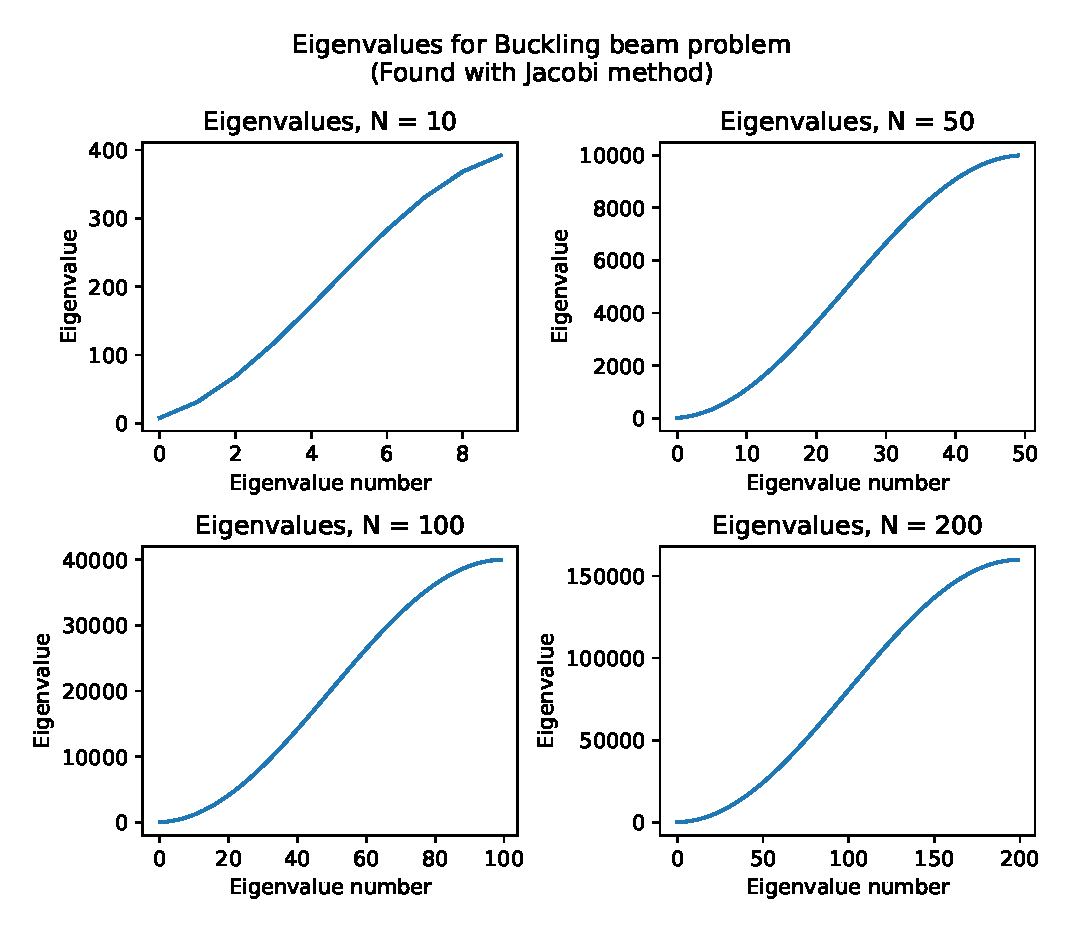
\includegraphics[width = 0.8\textwidth]{figures/eigvals_buckling_jacobi.eps}
    \caption{Eigenvalues for the buckling beam problem for different choices of dimension $N$. These values are calculated using the Jacobi method.}
    \label{fig:eigvals_buckling_jacobi}
\end{figure}
From the eigenvalue plot (\ref{fig:eigvals_buckling_jacobi}) we see qualitatively that the the curves follow a similar trend independent of N, but yet the y-axis change (Extends further for larger N). 
\begin{figure}[H]
    \centering
    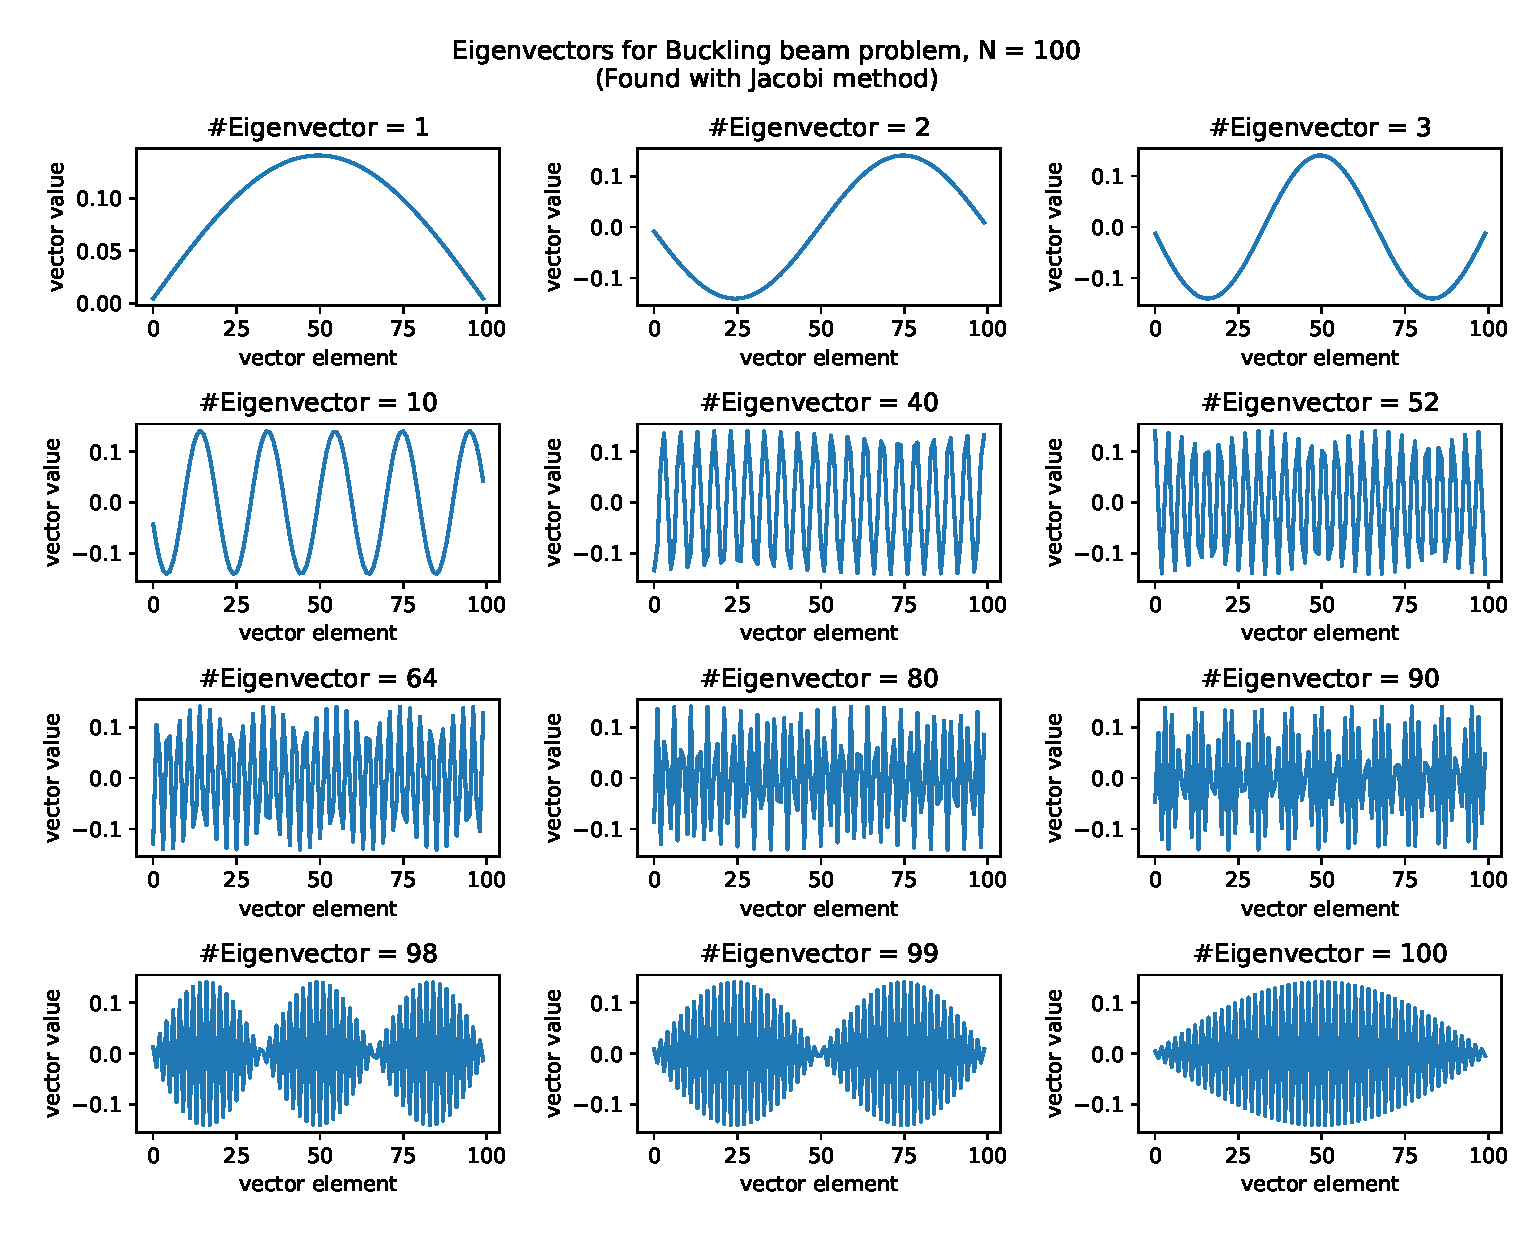
\includegraphics[width = \textwidth]{figures/eigvecs_buckling_jacobi.eps}
    \caption{Graphic display of the eigenvectors for the buckling beam problem for dimension $N = 100$ . The vector elements showed here are chosen such that it displays some of the more interesting wave patterns found among the 100 eigenvectors}
    \label{fig:eigvecs_buckling_jacobi}
\end{figure}
From the eigenvector plot (\ref{fig:eigvecs_buckling_jacobi}) we first of all notice a clear relation between the vector element number and then the number of tops on the curve. The vector element number seem to correspond directly to the number of tops on the curve. For higher vector element numbers, of 50 and above, we see a more complex wave pattern with multiple wave frequency changing during the increment of the vector element number. At the highest numbers (>90) this comes across like small wave packets. \\
In order to investigate the precision and efficiency of the Jacobi method we ran the algorithm for dimensions $N \in [2, 100]$ and calculated/measured the number of iterations, mean error (compared to analytical expression (\ref{eq:analytical_eigvals})) and finally the run time of the main algorithm. The relationship between these and dimension $N$ are shown in figure \ref{fig:iter_dim_jacobi}, \ref{fig:error_dim_jacobi} and \ref{fig:time_dim_jacobi}. In all of the cases we got quite good linear fits on the logarithmic plots.
\begin{figure}[H]
    \centering
    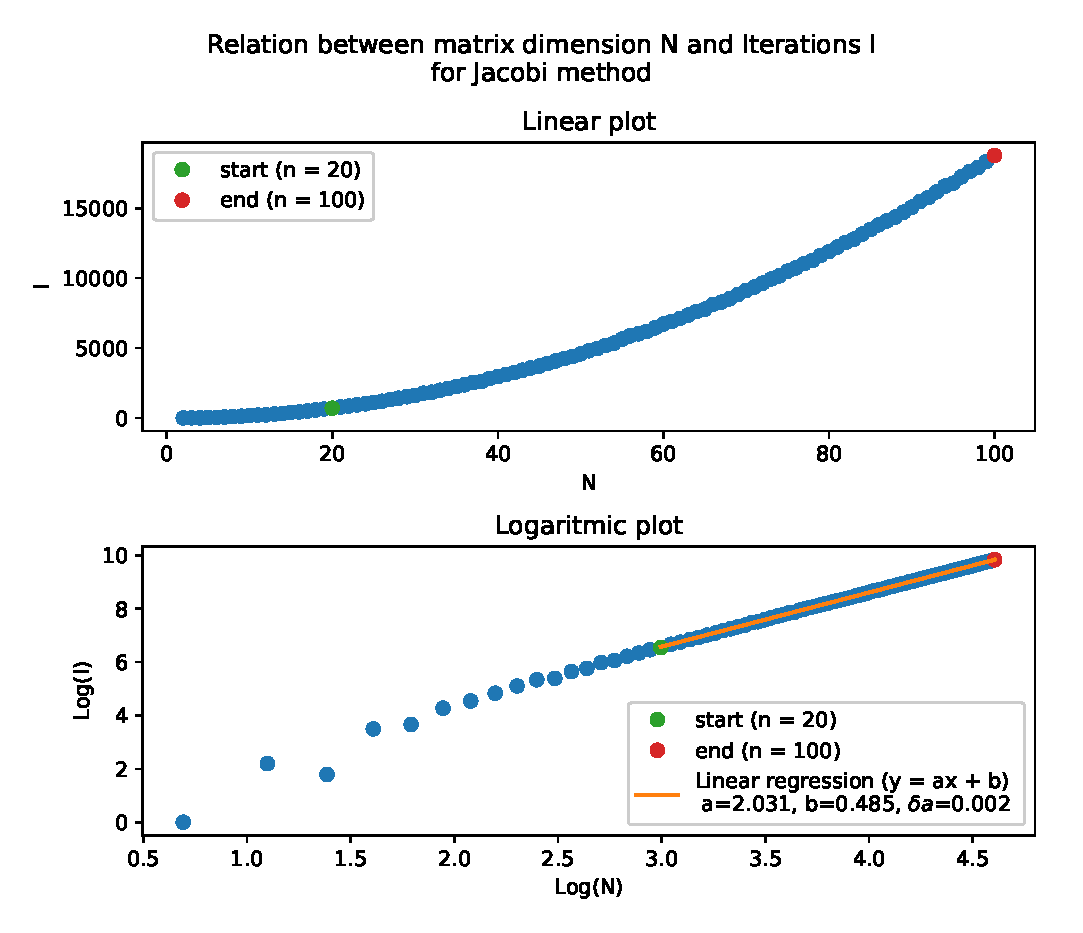
\includegraphics[width = \textwidth]{figures/iter_dim_jacobi.eps}
    \caption{Linear and logarithmic plot (with linear regression) of the iterations $I$ used in the Jacobi algorithm for different choices of dimension $N$}
    \label{fig:iter_dim_jacobi}
\end{figure}
On the iterations-dimension-plot (\ref{fig:iter_dim_jacobi}) we find that the iterations $I$ increase with N as:
\begin{align*}
    I(N) = 1.624 \cdot N^{2.031}
\end{align*}
\begin{figure}[H]
    \centering
    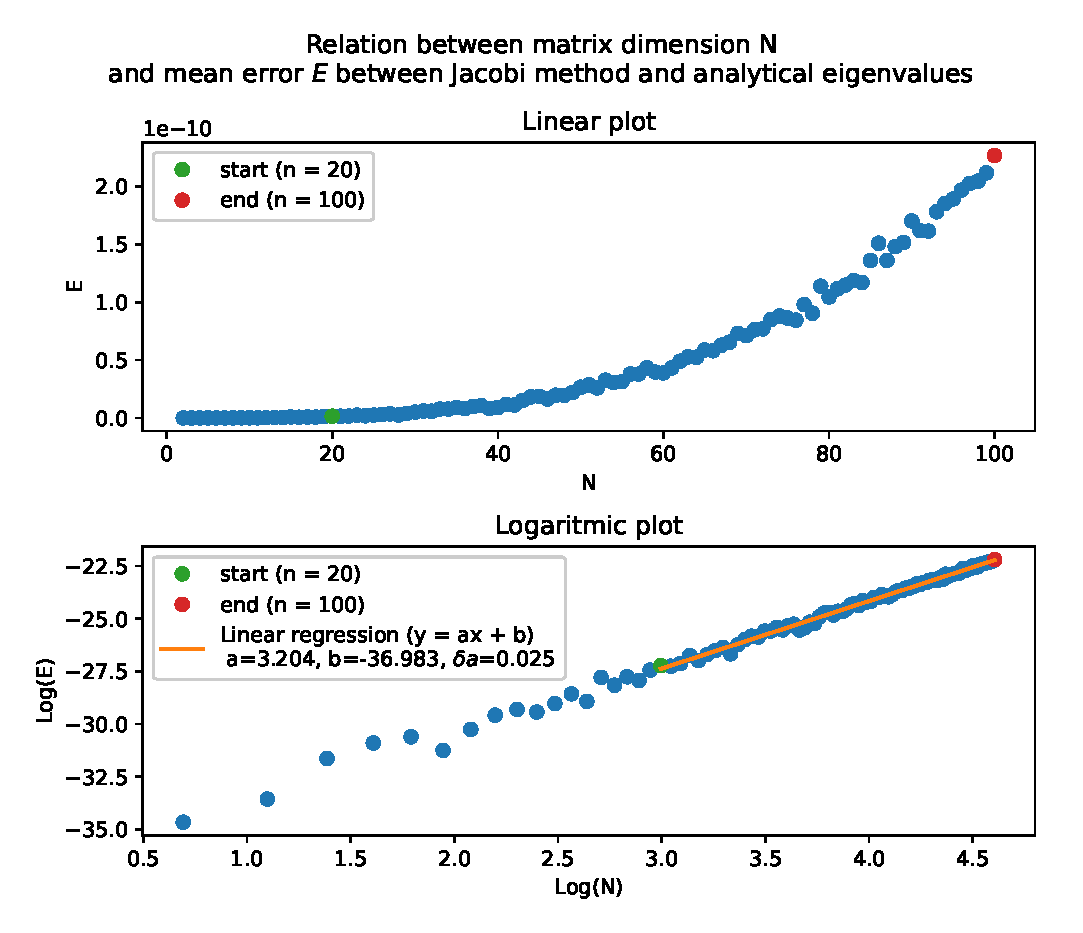
\includegraphics[width = \textwidth]{figures/error_dim_jacobi.eps}
    \caption{Linear and logarithmic plot (with linear regression) of the mean error $E$ for different choices of dimension $N$. The mean error is calculated as the mean difference of the numerical eigenvalues from the jacobi method and the analytical eigenvalues given with equation \ref{eq:analytical_eigvals}.}
    \label{fig:error_dim_jacobi}
\end{figure}
On the error-dimension-plot (\ref{fig:error_dim_jacobi}) we find that the mean error $E$ increase with N as:
\begin{align*}
    E(N) = E_0 \cdot N^{3.204}, \quad E_0 = \num{8.679e-17}
\end{align*}
\begin{figure}[H]
    \centering
    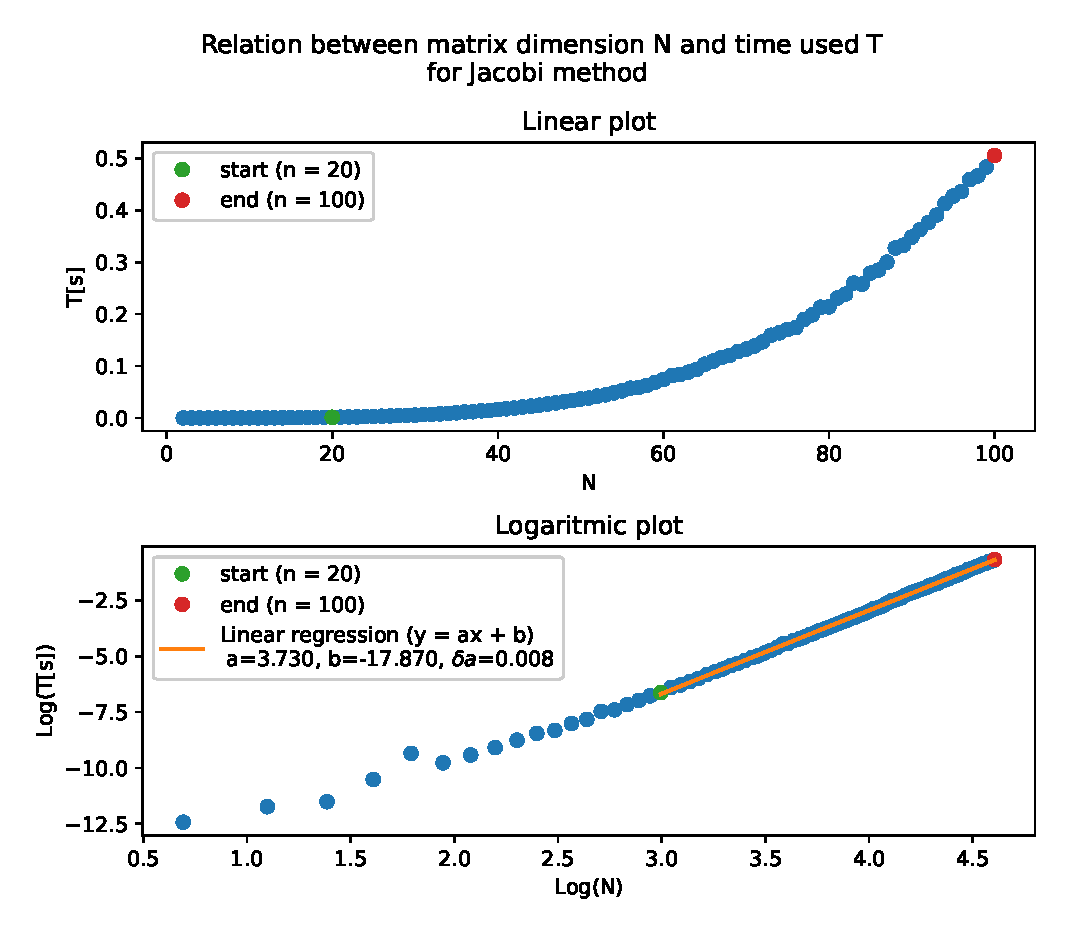
\includegraphics[width = \textwidth]{figures/time_dim_jacobi.eps}
    \caption{Linear and logarithmic plot (with linear regression) of the run time used for the main algorithm of the Jacobi algorithm for different choices of dimension $N$. Each run time is NOT an average value but since the program is called for increasing N with a python script, it produces quite stable results.}
    \label{fig:time_dim_jacobi}
\end{figure}
On the time-dimension-plot (\ref{fig:time_dim_jacobi}) wee find that the time $T$ increase with N as:
\begin{align*}
    T(N) = T_0 \cdot N^{3.730}, \quad T_0 = 0.01734 \ \mu \text{s}
\end{align*}

\newpage
\subsection*{Jacobi method with one electron}
Like for the buckling beam problem, figure \ref{fig:eigvals_buckling_jacobi}, we were able to plot the eigenvalues as a function of N
\begin{figure}[H]
    \centering
    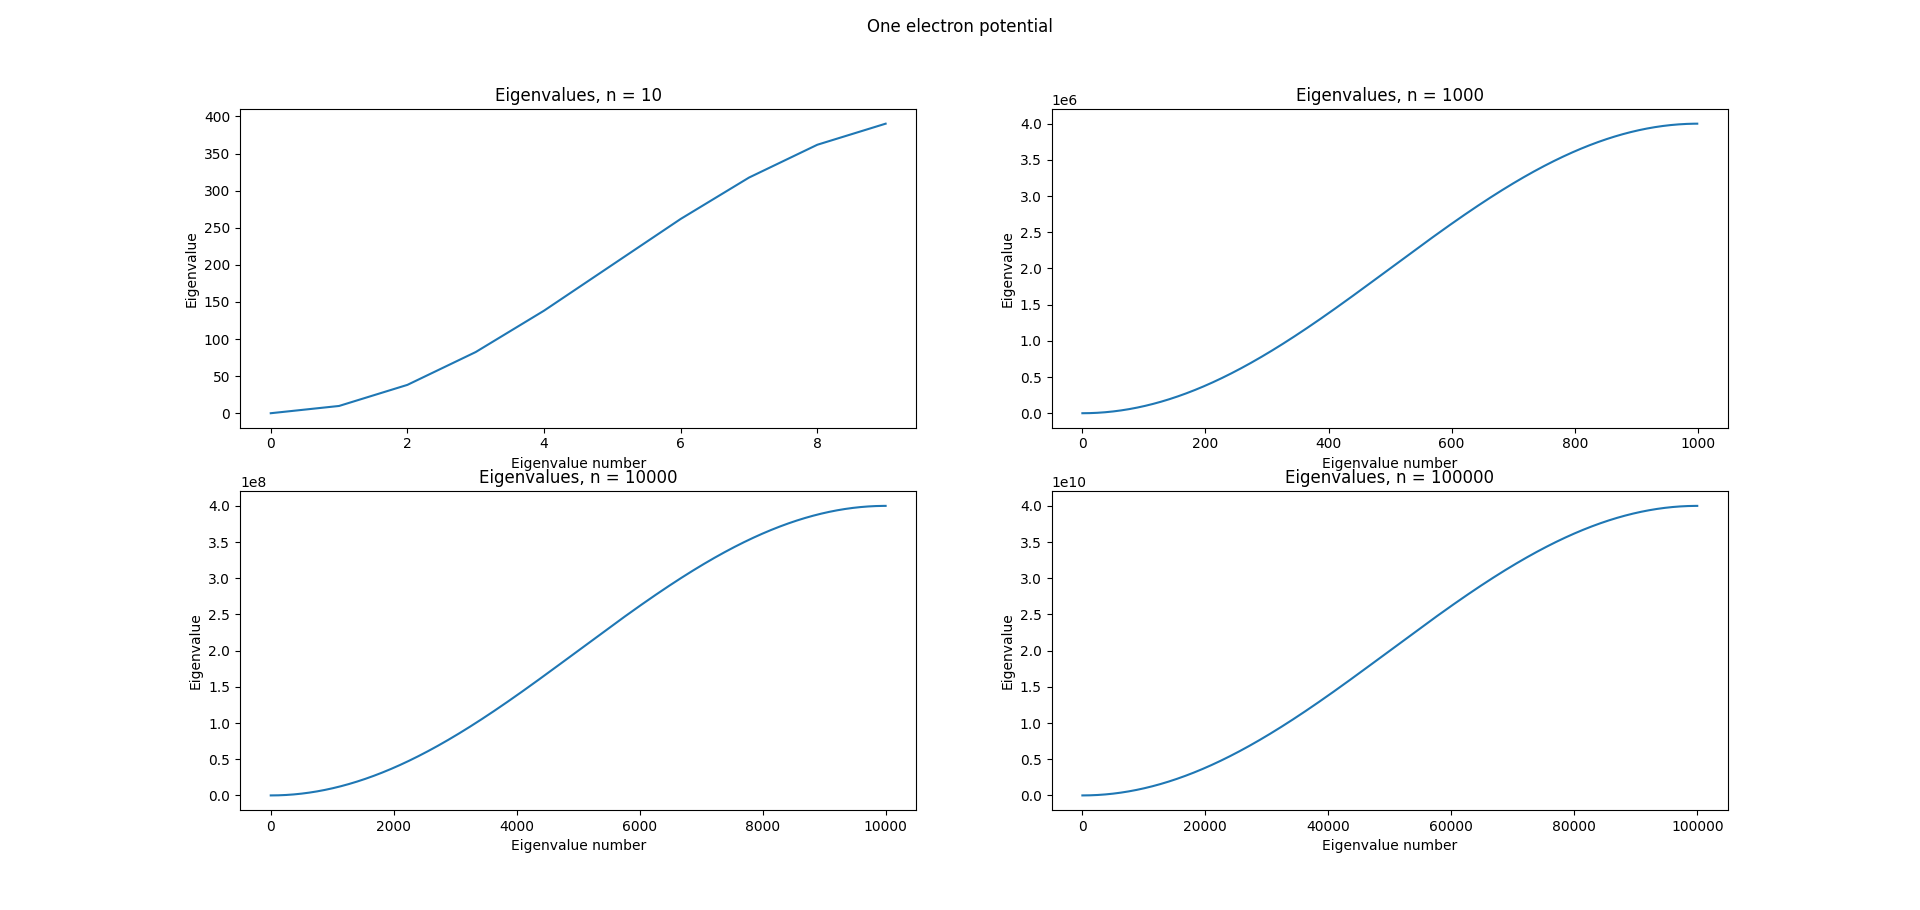
\includegraphics[width = \textwidth]{figures/eigvals_1e.png}
    \caption{Plot of eigenvalues as a function of N for the one electron potential}
    \label{fig:eigvals1}
\end{figure}
We found $\lambda_{1,2,3}$ to 4 leading digits with $N = 200$ integration points. We then tested  some values of $\rho_{max}$ for the best fit
\begin{table}[H]
    \centering
    \begin{tabular}{c|c|c|c}
        $\rho_{max}$ & $\lambda_1$ & $\lambda_2$ & $\lambda_3$ \\
        3 & 3.011 & 7.312 & 12.880 \\
        4 & 2.999 & 7.002 & 11.070 \\
        5 & 2.999 & 6.999 & 10.998 \\
        6 & 2.999 & 6.998 & 10.997 \\
        7 & 2.999 & 6.998 & 10.995 \\
    \end{tabular}
    \caption{Table showing how different values of $\rho_{max}$ impacted the precision of $\lambda$}
    \label{tab:rho1}
\end{table}
From the table we can see that the best fitted $\rho_{max}$ is equal to $5$.\\
We plotted the probability distribution and compared it to the buckling beam problem
\begin{figure}[H]
    \centering
    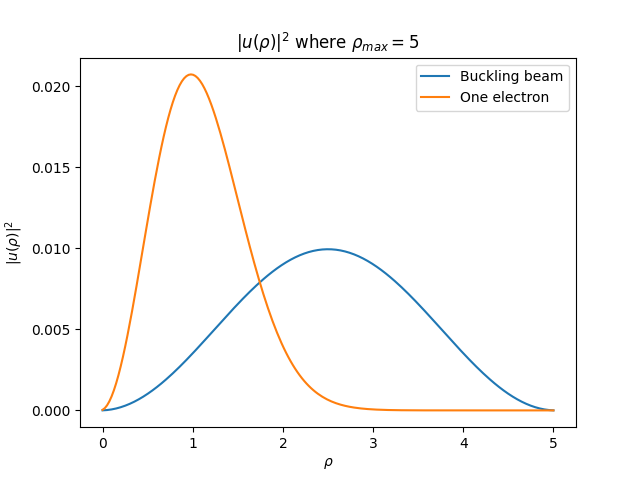
\includegraphics[width = \textwidth]{figures/eigvals_0and1e.png}
    \caption{The figure shows the ground state probability distribution of the one electron case and the buckling beam case.}
    \label{fig:eigvec01}
\end{figure} 
As the only difference between the methods is the additional potential we can see that the potential is forcing the electron to move closer to the origin of the spherical potential. 

\subsection*{Jacobi method with two electrons}
The first thing we need to do is calibrate $\rho_{max}$ so it gives us the correct eigenvalues and vectors. We do this by using the analytical eigenvalues calculated in a paper by M. Taut\cite{paper}. We can see that oscillator with strength $\Omega^2=0.25$ has eigenvalue $\lambda_{0.25} = 1.35$ and $\Omega^2=0.05$ has eigenvalue $\lambda_{0.05}=0.35$. We then found $\rho_{max}$ by trial and error using $N=200$.
\begin{table}[H]
    \centering
    \begin{tabular}{c|c|c}
         $\rho_{max}$ & $\lambda_{0.25}$ & $\lambda_{0.05}$ \\
         10 & 1.2498 & 0.3949 \\
         13 & 1.2496 & 0.3559 \\
         16 & 1.2494 & 0.3503 \\
         17 & 1.2494 & 0.3501 \\
         18 & 1.2493 & 0.3500 \\
         20 & 1.2491 & 0.3499 \\
    \end{tabular}
    \caption{Table showing how different values of $\rho_{max}$ impacted the precision of $\lambda$}
    \label{tab:rho2}
\end{table}
We will use $\rho_{max}=18$ as it is a good fit for both eigenvalues, and a very good fit for $\lambda_{0.05}$.
Like for the two previous cases we get a similar pattern for the two electron case
\begin{figure}[H]
    \centering
    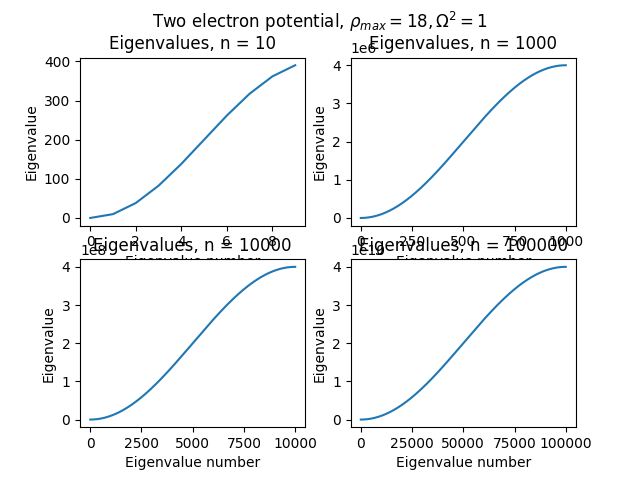
\includegraphics[width = \textwidth]{figures/eigvals_2e_1w.png}
    \caption{Plot of eigenvalues as a function of N for the two electron potential}
    \label{fig:eigvals2}
\end{figure}
We decided to plot the probability distribution for the following oscillator strengths $\Omega^2=[0.01, 0.5, 1, 5]$
\begin{figure}[H]
    \centering
    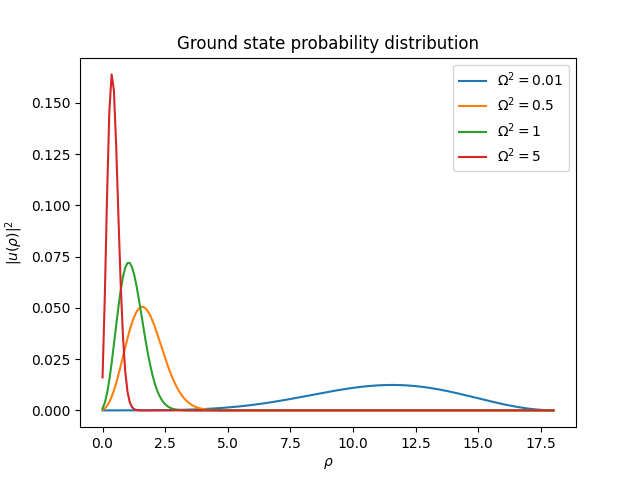
\includegraphics[width= \textwidth]{figures/eigvecs_2.png}
    \caption{Ground state probability distribution of the particles relative position}
    \label{fig:eigvecs2}
\end{figure}
We can see that stronger potential leads to the particles moving closer to the origin, while when the potential is very weak $\Omega^2=0.01$ we see that the particles move away from the origin.

\subsection*{Numerical performance}
Average time over 10 runs where $N=10,200$. The uncertainty is given by NumPy's standard deviation method (numpy.std)\cite{numpy}
\begin{table}[H]
    \centering
    \begin{tabular}{c|c|c|c|c}
        & $N=10$ & & $N=200$ &\\
        Method & Jacobi $\Bar{t}$ [s] & Armadillo $\Bar{t}$ [s] & Jacobi $\Bar{t}$ [s] & Armadillo $\Bar{t}$ [s]\\
        Buckling beam & 0.0025 \pm 0.0008 & 0.0006 \pm 0.0002 &13.68 \pm 0.04 & 0.10 \pm 0.03 \\
        One electron & 0.0021 \pm 0.0008 & 0.0008 \pm 0.0003 & 13.83 \pm 0.03 & 0.11 \pm 0.03\\
        Two electrons & 0.0009 \pm 0.0003 & 0.0008 \pm 0.0003 & 13.79 \pm 0.02 & 0.11 \pm 0.03
    \end{tabular}
    \caption{Average time with uncertainty, our Jacobi method vs Armadillos eig\_sym method}
    \label{tab:performance}
\end{table}



\section{Discussion}
\subsection{Jacobi method}
From the relation between iterations $I$, error $E$, time $T$ and dimension $N$ we found:
\begin{align*}
    &I(N) \approx \mathcal{O}(1.6N^2)&  &E(N) \approx \mathcal{O}(E_0N^{3.2})&  &T(N) \approx \mathcal{O}(T_0N^{3.7})&
\end{align*}
We must now ask ourselves how these numbers relate. The main loop for our Jacobi Algorithm look like this:
\begin{minted}{cpp}
    while (maxnondig > tol && iter <= maxiter){
        my_functions.JacobiRotate(A, Eigvec, p, q, n);
        my_functions.MaxOffdiag(A, p, q, maxnondig, n);
        iter++;
    }
\end{minted}
From our results we see that we generally use $\mathcal{O}(1.6N^2)$ runs through this loop for the off-diagonal element to converge to the specified tolerance ($\epsilon = \num{1e-10}$). Each Jacobi rotation, done by the function JacobiRotate, uses $\mathcal{O}(12n)$ FLOPs as marked here:
\begin{minted}{cpp}
    ...
    while (maxnondig > tol && iter <= maxiter){
          for (int i = 0; i < n; ++i){
            if (i != k && i != l){
              double a_ik_old = A(i,k);                 //3FLOPs
              double a_il_old = A(i,l);                 //3FLOPs
              A(i,k) = a_ik_old*cos - a_il_old*sin;
              A(k,i) = A(i,k);
              A(i,l) = a_il_old*cos + a_ik_old*sin;
              A(l,i) = A(i,l);
            }
        //eigenvectors
        double r_ik_old = Eigvec(i,k);
        double r_il_old = Eigvec(i,l);
    
        Eigvec(i,k) = r_ik_old*cos - r_il_old*sin;      //3FLOPs
        Eigvec(i,l) = r_ik_old*sin + r_il_old*cos;      //3FLOPs
        }
    }
\end{minted}
We do also calculate $\tau$, $\sin{\theta}$ and $\cos{\theta}$ for each rotation, but since this is outside the loop showed above, the contribution to the total number of FLOPs is negligible. But as we shall see next, the operations done in the Jacobi rotation is a factor $n$ smaller than the operations needed for finding the maximum off-diagonal element. In the function MaxOffdiag we go through a double for-loop:
\begin{minted}{cpp}
    double max;
    for (int i = 0; i < n; ++i){
        for (int j= i + 1; j < n; ++j){
            double aij = fabs(A(i,j));
            if (aij > max)
            {
            max = aij; p = i; q = j;
            }
        }
    }
  maxnondig = fabs(A(p,q));
\end{minted}
This requires $\frac{n(n-1)}{2} = \mathcal{O}(\frac{1}{2}N^2)$ FLOPs. Therefore we find that our implementation of the Jacobi method will require:
\begin{align*}
    \text{FLOPs}_{\text{Jacobi method}} = 1.6N^2 \cdot (6n + \frac{1}{2}n^2) = 9.6n^3 + 0.8n^4 = \mathcal{O}(0.8N^{4})
\end{align*}
We will expect the run time to be proportional with the number of FLOPs and we see that this is almost the case with $T(N)  \approx \mathcal{O}(T_0N^{3.7})$. The reason for the deviation could be explained by the fact that we did not look into memory fetching and other operations. \\
On figure \ref{fig:time_dim_armadillo} we see the run time results for the Armadillo eigenvalue solver (eig\_sym) is quite different than for the Jacobi method.
\begin{figure}[H]
    \centering
    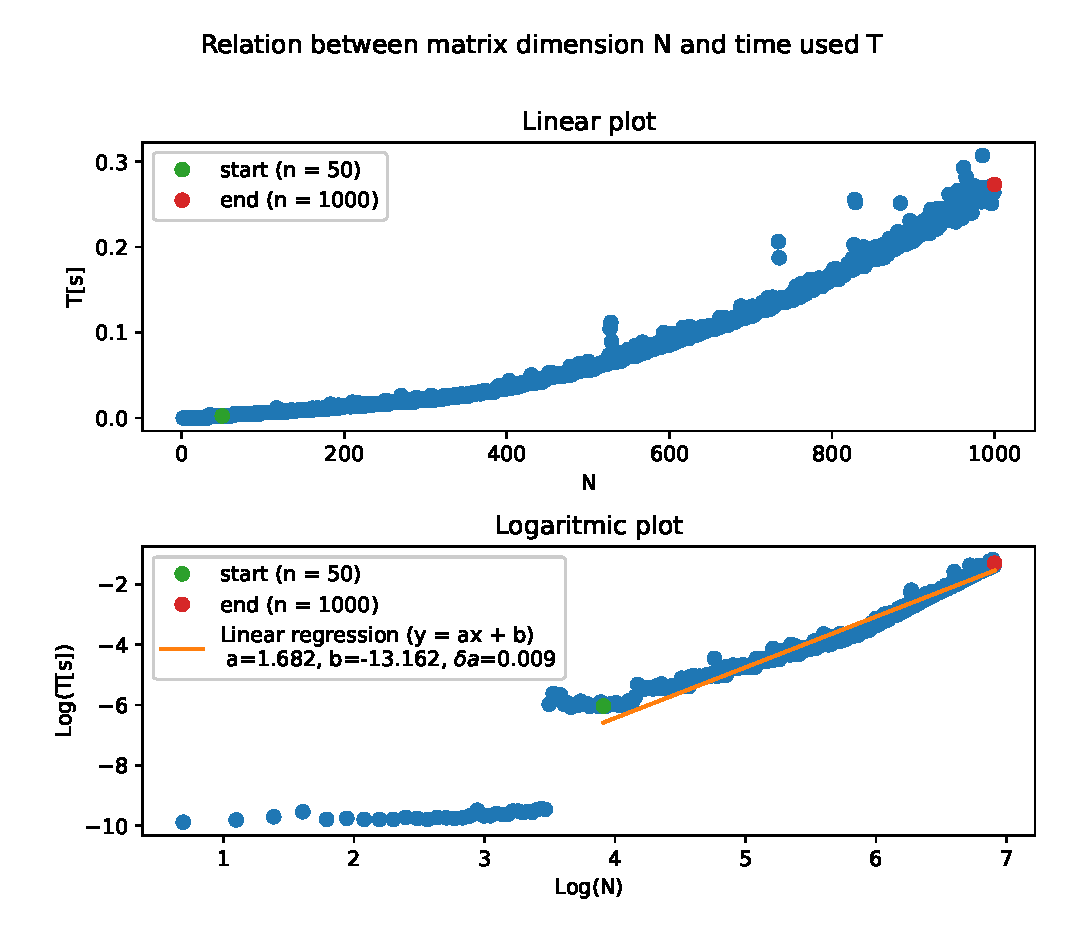
\includegraphics[width = \textwidth]{figures/time_dim_armadillo.eps}
    \caption{Linear and logarithmic plot (with linear regression) of the run time used for the Armadillo eigenvalue solver (eig\_sym) for different choices of dimension $N$}
    \label{fig:time_dim_armadillo}
\end{figure}
Here the linear regression on the logarithmic plot is not quite as fitting. Nonetheless we see that it is far more efficient regarding the run time which goes like:
\begin{align*}
    T_{\text{armadillo}}(N) \approx \mathcal{O}(N^{1.8})
\end{align*}
This does not come as a surprise since it is well established that the Jacobi method is not very efficient. \\
Another thing to notice about the efficiency of the Jacobi method is the increasing error of the eigenvalues. As shown already it increases as E_{\text{Jacobi}} = $\mathcal{O}(N^{3.2})$. The most reasonable explanation we have for this, is the accumulation of error due to numerical precision. The more similarity transformations we have to compute, the larger the accumulated error. Therefore it plays an important role whether the method uses converge fast or slow. We know that the Jacobi rotation can assign a value to a previous off-diagonal element set to zero, and thereby hinder convergence. But the increasing error is not purely a result of the Jacobi algorithm being ineffective. When performing the same investigation of error versus dimension with the more advanced armadillo eigenvalue solver (see figure \ref{fig:error_dim_armadillo}) we also see a similar trend:
\begin{figure}[H]
    \centering
    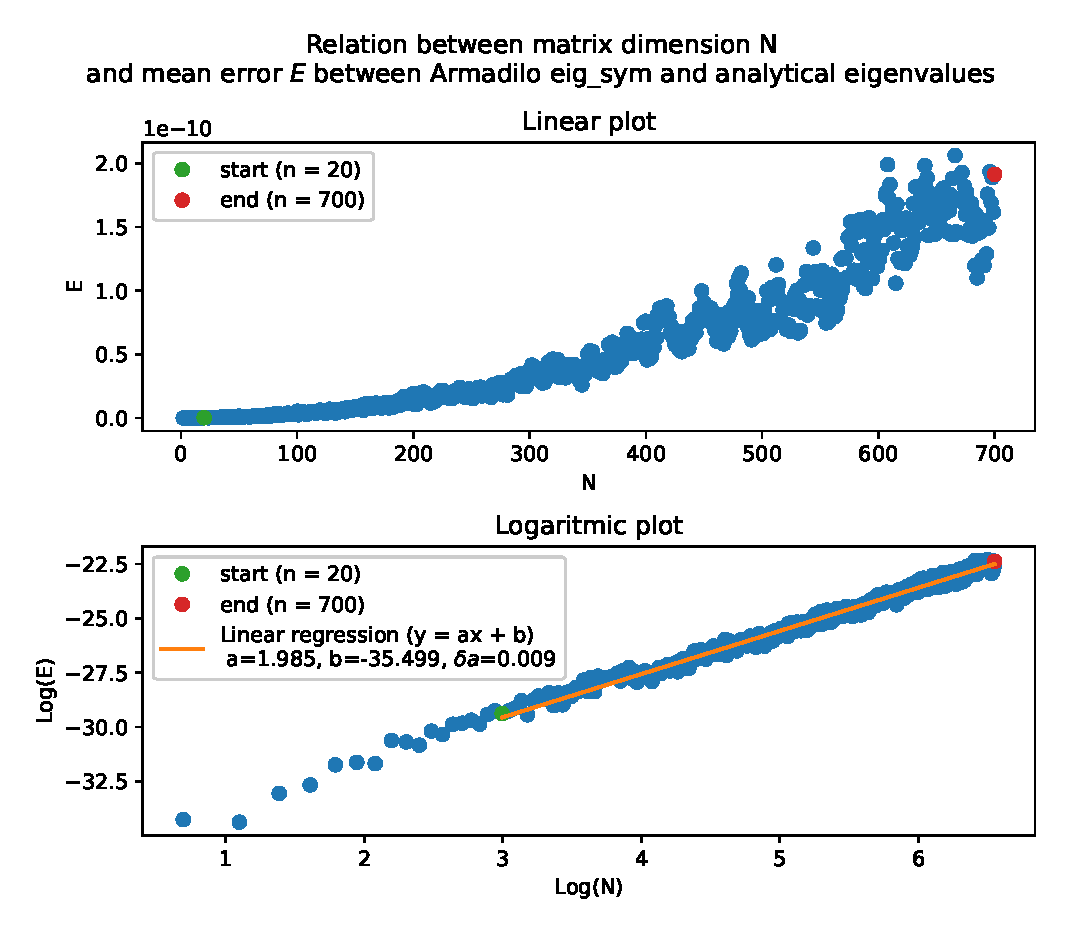
\includegraphics[width = \textwidth]{figures/error_dim_armadillo.eps}
    \caption{Linear and logarithmic plot (with linear regression) of the error for the Armadillo eigenvalue solver (eig\_sym) for different choices of dimension $N$}
    \label{fig:error_dim_armadillo}
\end{figure}
If we now go back to the root of the problem we remember that we used the approximation:
\begin{align*}
    u'' = \frac{u(\rho + h) - 2u(\rho) + u(\rho - h)}{h^2} + \mathcal{O}(h^2)
\end{align*}
From this one should expect that an increment of $N$ (decreasing $h$) would decrease the error with respect to the analytical expression. Since this is not the we must conclude that this is a property of the eigenvalue solver methods used. 

\subsection{Quantum mechanics, one and two electrons}
From figure \ref{fig:eigvecs2} we can see that higher oscillator strength makes the particles shift towards the origin, aswell as making their curve sharper. Since the curve is sharper the particles positions are better defined.\\
We can also see that for simulations with two electrons and weak potentials, e.g. $\Omega^2=0.01$, the Coulomb force starts to dominate. As a result the particles will repel each other, giving us a broader, more centralized curve.

\section{Conclusion}
During this project we have verified that the Jacobi method can be used successfully to solve eigenvalue problems such as the buckling beam problem or the quantum dots problem. We found that the number of iterations needed $I$, the mean error between numerical and analytical eigenvalues $E$, and a total run time of the main algorithm $T$ could be related to the dimension of the problem $N$ as:
\begin{align*}
    &I_{\text{Jacobi}}(N) \approx \mathcal{O}(1.6N^2)&  &E_{\text{Jacobi}}(N) \approx \mathcal{O}(E_0N^{3.2})&  &T_{\text{Jacobi}}(N) \approx \mathcal{O}(T_0N^{3.7})&
\end{align*}
By counting the FLOPs of the Jacobi algorithm we made a reasonable connection between the number of iterations needed and the run time. Further on we saw a general tendency for the error $E$ to increase both for the Jacobi method but also for the more advanced armadillo solver (eig\_sym). This lead us to the conclusion that both eigenvalue solvers introduces increasing errors for increasing $N$ due to numerical precision. For the Armadillo solver this went like:
\begin{align*}
    E_{\text{armadilo}} \approx \mathcal{O}(N^{2}), \quad T_{\text{armadilo}}(N) \approx \mathcal{O}(N^{1.8})
\end{align*}
Therefore at the end, the Jacobi method stands out as an extremely slow and ineffective method for solving the eigenvalue problem. Yet this has proven to be a successful method of gaining insight in various complex problems.

\newpage
\begin{thebibliography}{}
\bibitem{project1} Hoftun F. and Metzsch-Jensen M. (2020), \textit{Project 1}, Available at: \url{https://github.com/mikkelme/Project_1_FYS3150/blob/master/article%20/project1.pdf}
\bibitem{project_description} Univeristy of Oslo, Department of Physics (2020) \textit{Project 2 description} Available at: \url{https://github.com/CompPhysics/ComputationalPhysics/blob/master/doc/Projects/2020/Project2/pdf/Project2.pdf}
\bibitem{lecnotes7} Hjorth-Jensen, M. (2017) \textit{Diagonalization and eigenvalue problems}, Awailable at: \url{http://compphysics.github.io/ComputationalPhysics/doc/pub/eigvalues/pdf/eigvalues-print.pdf}
\bibitem{wiki:jacobi} Wikipeadia (2020) \textit{Jacobi Method}, Available at: \url{https://en.wikipedia.org/wiki/Jacobi_method} (Read: September 30th 2020)
\bibitem{paper} Taut M. (1993) {Two electrons in an external oscillator potential: Particular analytic solutions of a Coulomb correlation problem} \textit{Phys. Rev. A (48)} Available at: \url{https://journals.aps.org/pra/abstract/10.1103/PhysRevA.48.3561}
\bibitem{numpy} NumPy Documentation (2020), Available at: \url{https://numpy.org/doc/} (Read: September 30th 2020)
\bibitem{arma} Armadillo Documentation (2020), Available at: \url{http://arma.sourceforge.net/docs.html} (Read: Septemper 30th 2020)
\end{thebibliography}

\newpage
\section*{Appendix}
GitHub repository: \url{https://github.com/mikkelme/project2_FYS3150}


\subsubsection*{Proof that unitary transformations preserve orthogonality}
We have an orthogonal set of basis vectors $\vec{v_i}$ with $n \in \mathbb{N}$ vectors,
\begin{align*}
    \vec{v_i} = \begin{bmatrix}
    v_{i1} \\ v_{i2} \\ \vdots \\ v_{in}
    \end{bmatrix}
\end{align*}
Since the set is orthogonal we have
\begin{align*}
    \vec{v_j^T} \vec{v_i} = \delta_{ij}
\end{align*}
Where $\delta_{ij}$ is the Kronecker-delta\footnote{\url{https://en.wikipedia.org/wiki/Kronecker_delta}}.\\
For an unitary matrix $\vec{A}$ we have
\begin{align*}
    \vec{A}^* \vec{A} &= \vec{A}^{-1} \vec{A} = \vec{I}\\
    \vec{A}^* &= \overline{\vec{A^T}} = \vec{A}^{-1}
\end{align*}
If the matrix $\vec{A}$ is real then $\vec{A^T} =  \overline{\vec{A^T}}$ is an orthogonal matrix instead.
The orthogonality and the dot product is preserved if we do an orthogonal or unitary transformation. Here shown using an unitary matrix $\vec{A}$
\begin{align*}
    \vec{w_i} &= \vec{A} \vec{v_i}\\
    \vec{w_j} &= \vec{A} \vec{v_j}\\
    \vec{w_j^*} \vec{w_i} &= (\vec{A} \vec{v_j})^* \vec{A} \vec{v_i} = \vec{v_j}^* \vec{A}^* \vec{A} \vec{v_i} = \vec{v_j^*} \vec{I}\ \vec{v_i} =\vec{v_j^*} \vec{v_i} = \delta_{ij}
\end{align*}
This means that the orthogonality and the dot product is preserved when the vectors are transformed by an orthogonal or unitary matrix $\vec{A}$.

\subsubsection*{Proof that $\alpha$ has dimensions length}
\begin{align*}
    [m] &= \frac{[Js]^2}{kg^2 [1/s]^2}^{1/4}\\
    &= \frac{[kg^2 m^4 s^2 1/s^4 ]}{kg^2 [1/s]^2}^{1/4}\\
    &= {m^4}^{1/4} = [m]
\end{align*}
Similar proofs can be done for other dimensionless constants.


\end{document}
